\clearpage\null\vfill
\thispagestyle{empty}
\begin{minipage}[b]{.9\textwidth}
  \begin{center}
  \setlength{\parskip}{.5\baselineskip}
  {\color{phdcol0}%
   \ccLogo\hspace{.1cm}%
   \ccAttribution\hspace{.1cm}%
   \ccNonCommercial\hspace{.1cm}%
   \ccNoDerivatives}\hspace{.15cm}%
  \footnotesize%
  This work is licensed under {\color{phdcol1}\textbf{http://creativecommons.org/licenses/by-nc-nd/3.0/}}
  \end{center}
\end{minipage}
\vspace*{2\baselineskip}
\clearpage
\thispagestyle{empty}
\vspace*{\stretch{1}}
\begin{flushright}
  \textit{Ah, la thèse.}
\end{flushright}
\vspace*{\stretch{7}}
%
%%
%\chapter*{Remerciements}
%
%
%\`A tous, \textbf{merci infiniment} !
%
\chapter*{Résumé Long}

Cette thèse traite la résolution du problème de satisfaisabilité booléenne (SAT).
Le problème de satisfabilité est un problème important qui traite de problèmes importants dans différents domaines tels 
que la décision de planification~\cite{planning_92}, la biologie~\cite{biology_06}, la vérification de logiciel et de 
matériel informatique~\cite{biere1999symbolic}, de raisonnement automatique~\cite{heule2016solving}.
Leurs évolutions au cours des dernières décennies leur ont permis de traiter des problèmes de plus en plus complexes.
Dans un travail récent, des chercheurs ont réussi a prouver à l'aide d'un solveur SAT, une borne maximum
pour le problème de coloration des triplets pythagoriciens~\cite{heule2016solving}, avec une preuve de 200 TB.

Le principe de base de SAT est de déterminer si une formule propositionnelle
est satisfaisable, c'est à dire que toutes les contraintes peuvent être satisfaites,
ou insatisfaisable, c'est-à -dire qu'il n'y a aucun moyen de satisfaire toutes les contraintes avec une même affectation.
Ce calcul est effectué par un solveur SAT qui répond usuellement $\sat$ lorsque la formule est satisfaisable et $\unsat$ dans le cas
contraire. Le problème SAT a été le premier problème à avoir été prouvé NP-Complet. Cela signifie que
l'on ne connait pas d'algorithme capable de résoudre le problème avec une complexité polynomiale.
La résolution du problème est l'un des sept prix du millénaire, à savoir P = NP.

Malgré cette complexité, les solveurs SAT sont capables de résoudre de plus en plus de problèmes complexes.
Ce succès vient de l'introduction de différentes heuristiques sophistiquées et de 
l'algorithme de résolution, le $\guillemotleft$ Conflict Driven Clause Learning$\guillemotright$ (CDCL).
Il est basé sur l'algorithme nommé par ses auteurs Davis, Putnam, Logemann et Loveland (DPLL)\cite{dpll_62},
l'un des premier algorithme avec une utilisation non intensive de la mémoire.
%
%Cet algorithme est basé sur  
%et Loveland (DPLL)\cite{dpll_62}.
%
%
%l'optimisation de l'algorithme de
%résolution des conflits appelé $\guillemotleft$ Conflict Driven Clause Learning$\guillemotright$ (CDCL) qui est basée sur le premier
%algorithme (avec une utilisation non intensive de la  mémoire) nommé par ses auteurs Davis, Putnam, Logemann
%et Loveland (DPLL)\cite{dpll_62}.
\hakan{Enlever toutes la partie explicative de CDCL ?}
L'algorithme CDCL peut être vu sous forme de l'exploration d'un arbre binaire dans lequel  chaque branche représente 
une affectation. Il y a donc au total $2^n$ branches, avec $n$ le nombre de variables du problème.
Le principe de cet algorithme est d'explorer cet arbre binaire. 
La première étape consiste à choisir une variable dite de décision avec une polarité qui permet l'exploration
de l'arbre de recherche. Puis, d'effectuer les déductions logiques à partir de l'affection. 
Si l'algorithme découvre un conflit, c'est-à -dire que l'affectation courante n'est pas capable de satisfaire au moins une contrainte du problème, l'algorithme va calculer une clause dite de conflit qui permet d'élaguer 
cet espace de recherche qui ne contient pas de solution. Cette clause est une information redondante par
rapport au problème initial. Si aucun conflit n'est présent, l'algorithme choisit à nouveau une variable de décision. L'algorithme termine lorsque soit toutes les variables sont affectées auquel cas le problème 
est satisfait, soit un conflit est apparu avec uniquement des déductions logiques auquel cas le
problème est non satisfaisant.
La Figure~\ref{fig:cdclflow} présente sous forme d'un organigramme le fonctionnement de l'algorithme CDCL.

\begin{figure}[!htbp]
\begin{tikzpicture}[node distance=1.5cm,
,every node/.style={scale=0.7,fill=white, font=\sffamily}, align=center]
% Specification of nodes (position, etc.)
\tikzset{%	
	>={Latex[width=2mm,length=2mm]},
	% Specifications for style of nodes:
	base/.style = {rectangle, rounded corners, draw=black,
		minimum width=2cm, minimum height=1cm,
		text centered, font=\sffamily},
	question/.style = {base, diamond, fill=blue!15},
	unsat/.style = {base, fill=red!30,minimum width=3cm},
	sat/.style = {base, fill=green!30,minimum width=3cm},
	process/.style = {base, minimum width=2.5cm, fill=orange!15,
		font=\ttfamily},
}
\node (isfin) [question] {Variables toutes \\assignées ?};
\node (dec)     [process, below = of isfin]          {Choix variable \\ de decision};
\node (sdec)     [right = of dec]          {};
\node (idec) [left = of isfin]  {};
\node (prop)    [process, below = of dec ]          {Propagation unitaire};
\node (conf)    [question, below = of prop] { Conflit ?};
\node (confanalyse) [process, below = of conf] {Analyse du \\ conflit};
\node (learn) [process] at ($(prop) + (160pt, 0)$) {Apprentissage de la \\ clause de conflit};
\node (isend) [question] at ($(confanalyse) + (160pt, 0)$) {Niveau de \\decision zero ?};
\node (end) [unsat] at ($(isend) + (140pt, 0)$) {$\unsat$};
\node (ends) [sat] at ($(isfin) + (+160pt, 0)$){$\sat$};


\draw[->, thick]     (sdec) -- (dec);
\draw[->, thick]     (dec) -- (prop);
\draw[->, thick]     (prop) -- (conf);
\draw[->, thick]     (conf) -| node [yshift=5.5 cm] {non}(idec.center) -- (isfin);
\draw[->, thick]     (conf) -- node {oui} (confanalyse);
\draw[->, thick]     (isfin) -- node {non}(dec);
\draw[->, thick]     (confanalyse) --(isend);
\draw[->, thick]     (isend) -- node {oui}(end);
\draw[->, thick]     (isfin) -- node {oui}(ends);
\draw[->, thick]     (learn) -- (prop);
\draw[->, thick]     (isend) -- node [] {non}(learn);

\end{tikzpicture}
\caption{Organigramme de l'algorithme CDCL}
\label{fig:cdclflow}
\end{figure}

%\begin{figure}[!htbp]
%	\begin{tikzpicture}[node distance=1.5cm,
%	,every node/.style={scale=0.7,fill=white, font=\sffamily}, align=center]
%	% Specification of nodes (position, etc.)
%	\tikzset{%	
%		>={Latex[width=2mm,length=2mm]},
%		% Specifications for style of nodes:
%		base/.style = {rectangle, rounded corners, draw=black,
%			minimum width=2cm, minimum height=1cm,
%			text centered, font=\sffamily},
%		question/.style = {base, diamond, fill=blue!15},
%		unsat/.style = {base, fill=red!30,minimum width=3cm},
%		sat/.style = {base, fill=green!30,minimum width=3cm},
%		process/.style = {base, minimum width=2.5cm, fill=orange!15,
%			font=\ttfamily},
%	}
%	\node (isfin) [question] {All vars\\ assign?};
%	\node (dec)     [process, below = of isfin]          {Choose decision var};
%	\node (sdec)     [right = of dec]          {};
%	\node (idec) [left = of isfin]  {};
%	\node (prop)    [process, below = of dec ]          {Unit Propagation};
%	\node (conf)    [question, below = of prop] { IsConflict?};
%	\node (confanalyse) [process, below = of conf] {Conflict Analysis};
%	\node (learn) [process] at ($(prop) + (160pt, 0)$) {Learn conflict clause};
%	\node (isend) [question] at ($(confanalyse) + (160pt, 0)$) {is level\\zero?};
%	\node (end) [unsat] at ($(isend) + (140pt, 0)$) {$\unsat$};
%	\node (ends) [sat] at ($(isfin) + (+160pt, 0)$){$\sat$};
%	
%	
%	\draw[->, thick]     (sdec) -- (dec);
%	\draw[->, thick]     (dec) -- (prop);
%	\draw[->, thick]     (prop) -- (conf);
%	\draw[->, thick]     (conf) -| node [yshift=5.5 cm] {no}(idec.center) -- (isfin);
%	\draw[->, thick]     (conf) -- node {yes} (confanalyse);
%	\draw[->, thick]     (isfin) -- node {no}(dec);
%	\draw[->, thick]     (confanalyse) --(isend);
%	\draw[->, thick]     (isend) -- node {yes}(end);
%	\draw[->, thick]     (isfin) -- node {yes}(ends);
%	\draw[->, thick]     (learn) -- (prop);
%	\draw[->, thick]     (isend) -- node [] {no}(learn);
%	
%	\end{tikzpicture}
%	\caption{Organigramme de l'algorithme CDCL}
%	\label{fig:cdclflow}
%\end{figure}

Cependant certains problèmes présentent des symétries, certaines branches de l'espace de recherche 
sont donc équivalentes à la symétrie près. Prenons comme exemple le $\guillemotleft$problème des pigeons $\guillemotright$ dans lequel nous avons un ensemble de pigeons qui doivent êtres attribués à des nids différents. Dans ce problème il y a un nid de moins que le nombre de pigeons.
Le but de ce problème est de déterminer s’ il est possible d'attribuer un nid différent à chaque pigeon.
 La figure~\ref{fig:holefr} pressent une instance de ce problème.
 
 
 \begin{figure}[!htbp]
  \centering
  \begin{tikzpicture}[
  start chain = going right,
  node distance = 0pt,
  AStyle/.style={draw, minimum width=2em, minimum height=2em, 
   outer sep=0pt, on chain, fill=yellow!0!white}]
  \node [AStyle] (1) {\huge\textcolor{gray}{\PHdove}};
  \node [AStyle] (4) {\huge\textcolor{gray}{\PHdove}};
  \node [AStyle] (5) {\huge\textcolor{gray}{\PHdove}};
  \node [AStyle, draw] (6) {\huge\textcolor{gray}{\PHdove}};
  \node [ minimum width=2em, minimum height=2em, 
  outer sep=1pt, on chain] (7) {\huge\textcolor{gray}{\PHdove}};
  \end{tikzpicture}
  \caption{Représentation graphique d'une instance du problème des pigeons(5 pigeons, 4 nids)}
  \label{fig:holefr}
 \end{figure}
 
 
Pour un humain, la réponse à ce problème est évidente, mais un solveur de l'état de l'art va parcourir toutes 
les combinaisons possibles de couples (pigeon, nid), cela le mène à une explosion combinatoire.
Pour cette raison, résoudre ce problème avec un solveur s'avère très chronophage et même impossible dans des temps raisonnables
pour un nombre de pigeons supérieur à environ 15.
%Cependant, certains problèmes possèdent un espace de recherche énorme et ne peuvent pas 
%être traité par un solveur SAT. Un exemple d'un tel problème peut être le problème de tournées de véhicules (VRP). 
%Il s'agit du service d'entreprise de livraison, dans lequel étant donné une flotte de véhicules basés dans un dépôt, ceux ci doivent faire des rondes entre des clients qui ont demandés chacun une certaine quantité de marchandises. Le circuit effectué par un véhicule pour la visite de tous les clients
%est appelé la tournée du véhicule. L'objectif est de trouver la tournée qui minimise les coûts de livraison (monétaire, distance, temps, ....).
%
%
%Dans le problème précédent, renommer l'ensemble de véhicules identiques nous donnera exactement le même problème. C'est ce qu'on appelle une symétrie.
De manière plus  générale, une symétrie est une transformation qui laisse un objet (ou un aspect de l'objet) inchangé. Les symétries sont généralement définies comme une propriété syntaxique d'un problème lorsque leur présence est inhérente à l'encodage du problème.
Dans ce cas, une permutation des variables préserve la spécification originale du problème.
Dans le cas où les symétries sont indépendantes d'une représentation particulière du problème, il s'agit de symétries sémantiques.
La présence de symétrie dans un problème force l'algorithme de recherche à explorer en vain l'espace de recherche symétrique et entrave considérablement ses performances. La rupture de symétrie est une approche qui évite au solveur de visiter l'espace de recherche symétrique.
Pour pouvoir exploiter les symétries, la première étape consiste à les trouver. Dans le contexte de la satisfaction booléenne, la détection des symétries syntaxique se fait tout d'abord par la transformation de la spécification en un graphe coloré et ensuite à l'application d'un outil d'automorphisme de graphe sur celui-ci.
Différents outils traitent de ce problème dans l'état de l'art tel que $\bliss$~\cite{JunttilaKaski:ALENEX2007}, $\saucy$~\cite{katebi2010symmetry}, …

Lorsque les symétries sont obtenues à l'aide de ces outils, l'approche la plus courante pour les exploiter est d'utiliser une approche de rupture de symétrie statique. Elle est dite statique, car le traitement de cette approche  est effectuée avant la résolution du problème SAT.
Cette approche consiste à prendre le problème symétrique en entrée et à produire une formule à satisfaction équivalente en éliminant les symétries présentes. Le problème en sortie ne peut pas être insatisfaisable si le problème initial est satisfaisable.
Pour produire une formule équivalente sans présence de symétries, le problème est augmenté par des 
contraintes de rupture de  symétries ($\guillemotleft$symmetry breaking predicates $\guillemotright$ sbp). Celles-ci empêchent le solveur d'explorer l'espace de recherche symétrique. 
Autrement dit, si l'on considère notre exemple précédent avec les pigeons, le premier pigeon est attribué a un
exactement un nid, la symétrie est alors «cassé».
Plusieurs outils tels que $\shatter$~\cite{aloul06} et $\breakid$~\cite{devriendt2016improved}  utilisent cette technique pour accélérer le calcul du solveur en présence de symétries.
En général, cette approche apporte de bons résultats dans différentes instances symétriques, mais possède des défauts. Parmi eux, nous pouvons citer le nombre de contraintes ajoutées qui peut être exponentiel par rapport à la taille du problème, ce qui a pour conséquence de ralentir l'algorithme principal du solveur.
De plus, étant donné que ce calcul est effectué avant le lancement du solveur, cette approche peut être difficilement combiner avec d'autre technique de rupture de symétries. Aussi celui-ci ne peut pas distinguer les contraintes originales du problème avec les contraintes de rupture de symétrie. Avec cette information, le solveur peut modifier ces heuristiques pour augmenter ces performances. De plus, 
Pour ces raisons, certains problèmes avec de nombreuses symétries ne peuvent pas être traités avec cette approche.
Une autre approche dite rupture de symétrie dynamique consiste à utiliser les symétries durant l'algorithme de recherche du solveur SAT, plus précisément à modifier son comportement pour exploiter les propriétés de symétrie du problème. Cette approche consiste à déduire des faits symétriques par rapport aux déductions effectuées par le solveur. Lorsque ces faits sont ignorés, le solveur va explorer en vain l'espace de recherche symétrique.
Ces déductions réduisent le nombre de décisions qui sont des suppositions du solveur qui sont choisies de 
manière heuristique et augmentent le nombre de propagations qui sont les déductions logiques faites par le solveur. 
En d'autres termes, cette approche transforme les suppositions du solveur en déductions logiques.
Différents outils utilisent cette approche, nous pouvons cité parmi eux, \textit{Symmchaff}
qui exploite que certains types spécifiques de symétries, \textit{Symmetry Propagation (SP)}, \textit{Symmetry Learning Scheme (SLS)}, \textit{Symmetry Explanation Learning (SEL)} qui ajoutent les symétrique des
clauses apprises pour permettre les déductions symétriques.
Étant donné que cette approche est dynamique, il est possible pour le solveur 
d'intégrer des heuristiques spécifiques ou encore de combiner les différentes techniques de rupture de symétrie.

Cette thèse vise à améliorer l'existant et rendre les solveurs plus performants en présence de symétries et
propose différentes contributions allant dans ce sens.  

Notre première contribution consiste à mimer le comportement de la rupture de symétrie statique, mais 
opère dynamiquement, pendant l'exécution du solveur. On ajoute dans le solveur un composant de symétrie opportuniste qui va détecter que le solveur parcours un espace de recherche symétrique et va ajouter à celui-ci une contrainte appelée $\guillemotleft$ effectective symmetry breaking predicate $\guillemotright$ qui va empêcher le solveur de rester dans
l'espace de recherche symétrique. Cela a pour conséquence de réduire le nombre de contraintes et donc 
ne ralentit pas les solveur.
% Cette contrainte est dite effective, car 
% Ã  l'inverse de l'approche 
%de rupture de symétrie  statique la contrainte est forcément utilisée par le solveur. Aucune contrainte
%inutile n’est insérée dans le solveur. 
Ce composant de symétrie est fourni sous forme d'une bibliothèque codée en C++ et se nomme $\libdsb$.
Elle peut s'interfacer avec n'importe quelle solveur de type CDCL. 
Pour conduire nos expériences, nous l'avons interfacé avec un solveur de l'état de l'art nommé $\minisat$~\cite{een2003extensible}. Au total, l' intégration d’ $\libdsb$ ajoute environ 60 lignes de code 
et augmente de code de $\minisat$ de 3\%.
$\libdsb$ est open source fournit sous la licence GPLv3 et est disponible sur Github à l'adresse suivante: \url{https://github.com/lip6/cosy}.

Pour évaluer notre approche, nous avons comparé une version du solveur $\minisat$ combiné avec la bibliothèque $\libdsb$, que nous avons appelé $\cdclsym$ avec les solveurs de l'état de l'art.
Ces expérimentations se sont effectuées sur les instances de la SAT Competiton~\cite{jarvisalo2012international} sur les six dernières années de 2012 à 2017 où $\bliss$ a réussi a trouver des symétries. Au total, nous avons obtenue 1350 instances.
La figure~\ref{fig:frcactus} nous montre les résultats obtenus sous forme d'un cactus plot, 
dans lequel l'axe des abscisses nous montre le nombre d'instances réussi par chacun des solveurs et l'axe des ordonnées nous montre le temps de calcul des solveurs.
Nous avons conduit ces expériences avec deux outils d'automorphisme de graphe, à savoir 
 $\saucy$ Ã  gauche de la figure et $\bliss$ Ã  droite de la figure. 
 
Comme nous pouvons le constater, les résultats sont meilleurs  avec l'utilisation de l'outil d'automorphisme de 
graphe $\bliss$. La principale différence entre les deux outils est le nombre de permutations obtenues.
 $\bliss$ nous donne plus de permutations que $\saucy$, cela permet a notre outil $\cdclsym$ d'atteindre 
un nombre d'instances résolues de 775 alors que le deuxième meilleur outil $\breakid$ atteint un nombre d'instances résolues de 749 avec $\bliss$. Toutes les expériences étaient limité avec une durée de 5000 secondes.
Ces expériences nous démontrent que notre approche est aussi performante que les approches de ruptures de symétries statiques.
\begin{figure}[!htbp]
 \centering
 \subfloat[with \saucy]{{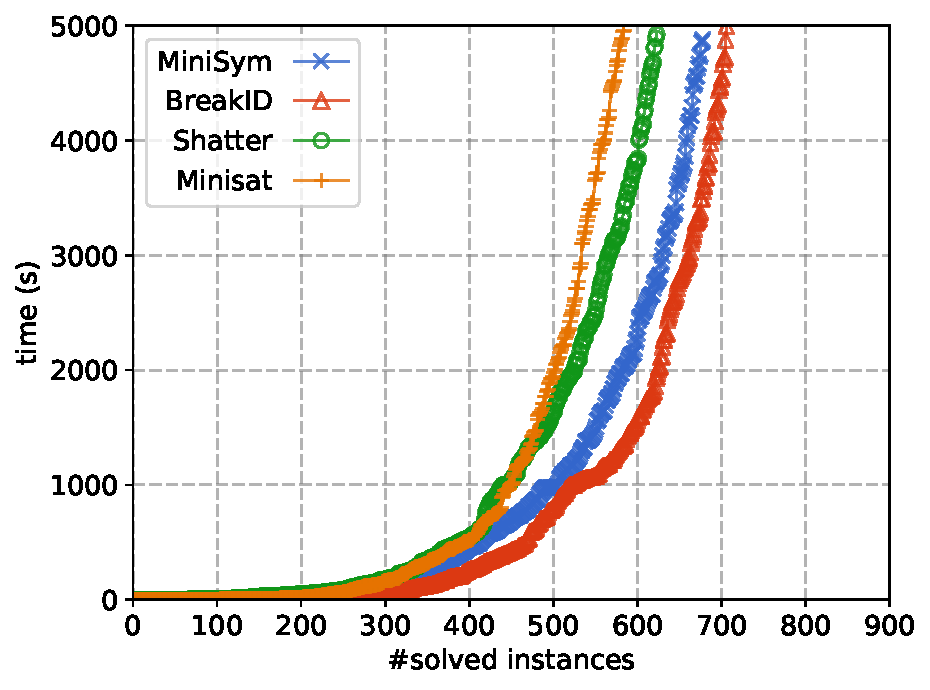
\includegraphics[scale=0.36]{img/saucy-result}}}%
 \qquad
 \subfloat[with \bliss]{{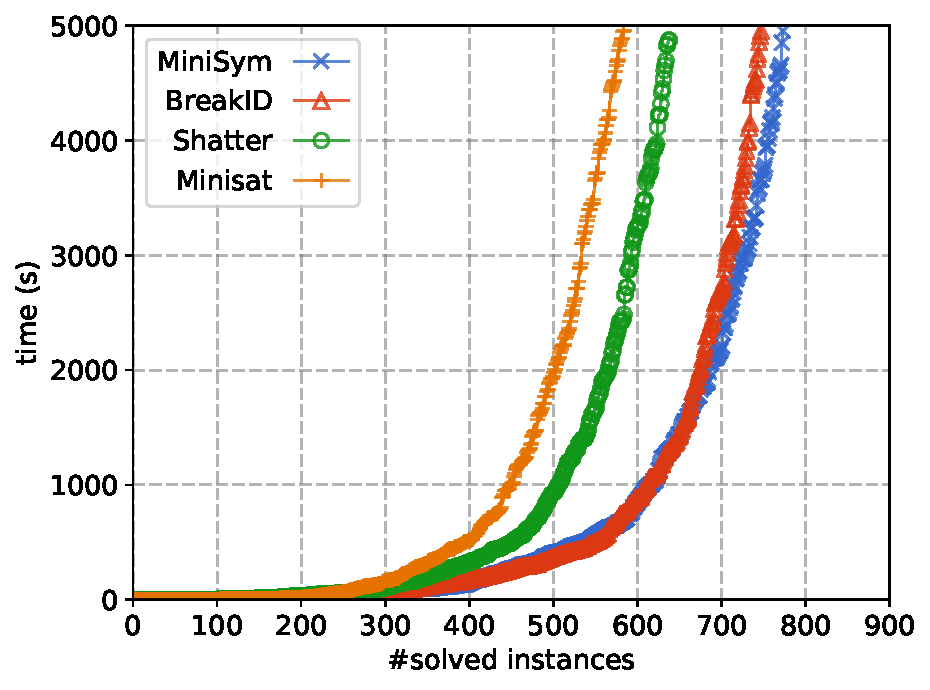
\includegraphics[scale=0.36]{img/bliss-result}}}%
 \caption{cactus plot  total number of instances}%
 \label{fig:frcactus}%
\end{figure}
Malgré les très bons résultats obtenus par notre approche certains problèmes qui sont résolus très 
rapidement les approches de rupture de symétrie dynamique tel que  Symmetry Propagation (SP) ne peuvent pas être traité par notre approche et vise versa.
SP est une approche qui a pour but d'accélérer la traversée de l'espace de recherche en déduisant des faits symétriques à partir des déductions effectuées par le solveur.
 À l'inverse notre approche consiste à éliminer les espaces de recherche 
symétriques. %Ces deux approches sont donc orthogonales.
Notre deuxième contribution consiste à déterminer si cette combinaison est possible qui se résume donc à la question suivante:
Est-il possible d'accélérer la traversée de l'espace de recherche tout en éliminant l'espace de symétrique ?
Pour que cette approche soit correcte, la contrainte qu'il faut absolument respectée est que la symétrie utilisée pour déduire les
faits symétriques doit être valide dans le problème actuel. Effectivement les clauses ajoutées pour éliminer l'espace de recherche
symétrique vont casser celle-ci qui ne peut donc plus être utilisée pour propager les faits symétriques.
L'approche naïve qui consiste à enlever les symétries dès lors qu'une contrainte de rupture de symétrie est ajoutée. Le problème avec cette approche est que l'ensemble vide est très vie atteint et donc plus aucune déduction symétrique ne peux être faites. Notre approche consiste à traquer les clauses utilisées par le solveur et à connaitre à tout instant l'ensemble des symétries valide grâce à l'introduction dite de symétrie locale pour chaque clause.
\begin{table}[!htbp]\footnotesize
 \centering
 \resizebox{1 \textwidth}{!}{
 \begin{tabular}{l|ccc}
  \toprule
  Benchmark  &\texttt{minisat-Sp} & \texttt{minisat-Sym} & \texttt{minisat-SymSP}\\
  \hline 
  Permutations 0–20 (704) & 194&197&\cellcolor{gray!30,}\textbf{198}\\
  Permutations 20–40 (136) & 33&\cellcolor{gray!30}\textbf{34}&\cellcolor{gray!30}\textbf{34}\\
  Permutations 40–60 (141) & 28&28&\cellcolor{gray!30}\textbf{29}\\
  Permutations 60–80 (168) & \cellcolor{gray!30}\textbf{65}&64&\cellcolor{gray!30}\textbf{65}\\
  Permutations 80–100 (51) & 28&\cellcolor{gray!30}\textbf{34}&\cellcolor{gray!30}\textbf{34}\\
  Permutations  \textgreater100 (200) & 58&59&\cellcolor{gray!30}\textbf{60}\\
  \hline 
  TOTAL no dup (1400) & 406 & 416 & \cellcolor{gray!30,}\textbf{420}\\
  \bottomrule
 \end{tabular}
 }
 \caption{Comparaison des approches sur les instances SAT.}
 \label{tab:satfr}
\end{table}%

\begin{table}[!htbp]\footnotesize
 \centering
 \resizebox{1 \textwidth}{!}{
 \begin{tabular}{l|ccc}
  \toprule
  Benchmark  &\texttt{minisat-Sp} & \texttt{minisat-Sym} & \texttt{minisat-SymSP}\\
  \hline 
  Permutations 0–20 (704) & \cellcolor{gray!30,}\textbf{233}&220&226\\
  Permutations 20–40 (136) & 50&\cellcolor{gray!30}\textbf{54}&\cellcolor{gray!30}\textbf{54}\\
  Permutations 40–60 (141) & 75&\cellcolor{gray!30}\textbf{83}&\cellcolor{gray!30}\textbf{83}\\
  Permutations 60–80 (168) & \cellcolor{gray!30}\textbf{11}&\cellcolor{gray!30}\textbf{11}&10\\
  Permutations 80–100 (51) & \cellcolor{gray!30}\textbf{11}&\cellcolor{gray!30}\textbf{11}&\cellcolor{gray!30}\textbf{11}\\
  Permutations \textgreater100 (200) & 90&\cellcolor{gray!30,}\textbf{109}&107\\
  \hline 
  TOTAL no dup (1400) & 470&488&\cellcolor{gray!30,}\textbf{491}\\
  \bottomrule
 \end{tabular}
 }
 \caption{Comparaison des approches sur les instances UNSAT.}
 \label{tab:unsatfr}
\end{table}
les expérimentations pour évaluer les performances de l'approche se sont effectuées sur les instances de la SAT Competiton sur les sept dernières années de 2012 à 2018 où $\bliss$ a trouver des symétries. Au total, nous avons obtenue un total de 1400 instances. 
Les tables \ref{tab:satfr} et \ref{tab:unsatfr} présentent respectivement
les résultats obtenues four les problèmes $\sat$ et $\unsat$.
La première colonne de chaque tableau énumère les classes de problèmes sur lesquelles nous avons effectué nos expériences: nous classons les problèmes en fonction du nombre de symétries qu'ils admettent. Une ligne notée "permutations X-Y (Z)" regroupe les problèmes Z ayant entre X et Y générateurs (symétries). Les autres colonnes indiquent le nombre de problèmes résolus par chaque approche. Les trois solveurs comparés sont respectivement
\texttt{minisat-Sp}, le solveur $\minisat$ avec l'approche SP; \texttt{minisat-Sym} le solveur $\minisat$ avec $\libdsb$ et \texttt{minisat-SymSP} le solveur avec l'approche combiné.
Globalement, nous observons que l'approche combinée est efficace dans de nombreuses classes de problèmes symétriques. Pour les problèmes de SAT, la combinaison a de meilleurs résultats que les deux autres approches (4 problèmes de SAT en plus par rapport au meilleur des deux autres). Lorsqu'on examine les problèmes de l'UNSAT, les résultats sont plus mitigées. Cela est du au coût mis en place pour maintenir a jour les structures
de chacun des deux approches de manière indépendante.
Cependant l'approche combiné apporte de meilleure résultats dans le nombre total d'instances résolues.
%Cette deuxième contribution réponds à la question, Est-il possible d'accélérer la traversée de l'espace de recherche tout en éliminant l'espace de symétrique ?
%La réponse est positive grâce à l'introduction des symétries locales. 
\chapter*{Abstract}
Nowadays, logic is omnipresent and it is used in different domains such as logic optimization, test pattern generation, formal verification and functional simulation, etc
One method to solve this kind of problem is satisfiability problem (SAT).
SAT solvers are more and more powerful and can handle large problems which seemed to be infeasible 
few years ago. However, some problems present symmetries which force the solver to explore fruitlessly
the symmetric part of the search space and hinders the performance. 
In this thesis, we set out to exploit symmetry properties of the problems in better way.
For this purpose, we create two majors contributions that aims to improve the state-of-the-art techniques and augment the number of solved instances. With an evaluation over the instances presented in the SAT competition, we show that our approach overcomes the state-of-the-art one and allow to solve more instances. 